%%%%%%%%%%%%%%%%%%%%%%%%%%%%%%%%%%%%%%%%%%%%%%%%%%%%%%%%%%%%%%%%%%%%%%%%%%%%%%%%
\chapter{Merging Placement and Re-embedding}
\label{ch:merge}
%%%%%%%%%%%%%%%%%%%%%%%%%%%%%%%%%%%%%%%%%%%%%%%%%%%%%%%%%%%%%%%%%%%%%%%%%%%%%%%%

In the previous chapters we have described several algorithms that deal with the
microarray layout problem in the traditional way: partitioning, placement and
re-embedding. The problem with the ``place and re-embed'' approach is that once
the placement is fixed, there is usually little freedom for optimization by
re-embedding the probes. Intuitively, better results should be obtained when the
placement and embedding phases are considered simultaneously instead of
separately. However, because of the generally high number of embeddings of each
single probe, it is not easy to design algorithms that efficiently use the
additional freedom and run reasonably fast in practice. In Chapter
\ref{ch:part}, we have shown how Pivot Partitioning successfully exploits this
extra freedom to outperform previous partitioning algorithms.

In this chapter, we describe the first placement algorithm that simultaneously
places and re-embeds the probes. Our goal was to design an algorithm that is
similar to the Greedy placement algorithm (Section \ref{sec:placement_greedy}),
so that we can make a better assessment of the gains resulting from merging the
placement and re-embedding phases.

%%%%%%%%%%%%%%%%%%%%%%%%%%%%%%%%%%%%%%%%%%%%%%%%%%%%%%%%%%%%%%%%%%%%%%%%%%%%%%%%
\section{\Greedyplus}
\label{sec:merge_greedyplus}

\Greedyplus\ \citep{Carvalho2007} is similar to Greedy in many respects. Spots
are filled in a greedy fashion, sequentially, using a user-configurable
$k$-threading pattern. For each spot $s$, \Greedyplus\ looks at $Q$ probe
candidates and chooses the one that can be placed at $s$ with minimum cost. The
main difference is that \Greedyplus\ considers all possible embeddings of a
candidate $p$ instead of only $p$'s given embedding. This is done by temporarily
placing $p$ at the spot $s$ and using OSPE (Section~\ref{sec:reembed_ospe}) to
compute $p$'s optimal embedding with respect to the already-filled neighbors of
$s$. (Naturally, OSPE can be used to compute the optimal embedding with respect
to border length or conflict index.) Another difference is that, unlike Greedy
and Row-Epitaxial, \Greedyplus\ does not assume that an initial embedding of the
probes is given.

Compared to Greedy, \Greedyplus\ spends more time evaluating each probe
candidate $p$ for filling a spot $s$. While Greedy takes $O(T)$ time to compute
the conflict index or the border length resulting from placing $p$ at $s$,
\Greedyplus\ requires $O(\ell \cdot T)$ time since it uses OSPE (recall that
$\ell$ is the probe length and $T$ is the deposition sequence length). We must
therefore use lower numbers $Q$ of candidates per spot to achieve a running
time comparable to Greedy.

There are three observations that significantly reduce the time spent with OSPE
computations when several probe candidates are considered in succession for
filling the same spot. First, we note that the $U_t$ and $M_{i,t}$ costs of OSPE
(Equations \ref{eq:ospe_ucost} and \ref{eq:ospe_mcost}, respectively) need to be
computed only once for a given spot $s$ since they do not depend on the probe
placed at $s$ but rather on the probes placed at neighbors of $s$: $U_t$ depends
solely on the neighbors of $s$, whereas $M_{i,t}$ depends on the neighbors of
$s$ and on the number $i$ of bases probe $p$ already contains at synthesis step
$t$ (if all probes have the same length $\ell$, then $c$ and $\theta$ in
Equation \ref{eq:ospe_mcost} are constants).

Second, once we know that a probe candidate $p$ can be placed at the spot $s$
with minimum cost $\kappa$, we can stop the OSPE computation for another
candidate $p'$ as soon as all values in a row of OSPE's dynamic programming
matrix are greater than or equal to $\kappa$.

Finally, we note that if two probe sequences $p$ and $p'$ share a common prefix
of length $r$, the first $r + 1$ rows of OSPE's matrix $D$ will be identical.
Hence, if we have previously calculated the minimum cost of $p$, we can speed up
the calculation of the minimum cost of $p'$ by skipping the first $r + 1$ rows
of $D$. In order to fully exploit this fact, we must examine the probes in
lexicographical order so that we maximize the length of the common prefix
between two consecutive probe candidates. For this reason, \Greedyplus\ uses the
same technique used by Greedy: Initially, the probe sequences are sorted
lexicographically and stored in a doubly-linked list. Once a probe $p$ is
selected to fill the current spot, it is removed from the list. For the next
spot to be filled, \Greedyplus\ looks at $Q$ probes in the list around $p$'s
former position, e.g., at $\lfloor Q/2 \rfloor$ probes to the left and at
$\lceil Q/2 \rceil$ probes to the right of $p$ (the list is traversed from left
to right).

%%%%%%%%%%%%%%%%%%%%%%%%%%%%%%%%%%%%%%%%%%%%%%%%%%%%%%%%%%%%%%%%%%%%%%%%%%%%%%%%
\section{Results}
\label{sec:merge_results}

\begin{table}[p!]\centering
\caption{\label{tab:greedyplus_nbl}
  Normalized border length (NBL) of layouts produced by \Greedyplus\ on random
  chips with varying number $Q$ of candidates per spot and amplitude of
  $k$-threading. Running times are reported in minutes.}
\footnotesize{
\begin{tabular}{crcrlcrlcr}
\vspace{1pt}
     &     & \multicolumn{2}{c}{$Q=500$} & & \multicolumn{2}{c}{$Q=1\,000$} & & \multicolumn{2}{c}{$Q=2\,000$} \\ \cline{3-4} \cline{6-7} \cline{9-10}
\vspace{1pt}
Dim. & $k$ & NBL & Time & & NBL & Time & & NBL & Time \\
\hline
$300\times 300$ &  0 &      17.9356  &  5.4 &  &      17.7136  & 10.6 &  &      17.5460  &  20.6 \\
                &  1 &      18.0922  &  5.4 &  &      17.8988  & 10.5 &  &      17.7501  &  20.4 \\
                &  2 &      17.9886  &  5.4 &  &      17.7905  & 10.5 &  &      17.6342  &  20.5 \\
                &  3 &      17.9339  &  5.7 &  &      17.7406  & 10.5 &  &      17.5799  &  20.5 \\
                &  4 &      17.8978  &  5.7 &  &      17.7155  & 11.1 &  &      17.5506  &  20.5 \\
                &  5 &      17.8862  &  5.7 &  &      17.7013  & 10.6 &  &      17.5359  &  20.5 \\
                &  6 &      17.8749  &  5.4 &  &      17.6908  & 10.6 &  &      17.5225  &  20.5 \\
                &  7 &      17.8641  &  5.5 &  &      17.6807  & 10.6 &  &      17.5223  &  20.6 \\
                &  8 &      17.8605  &  5.4 &  &      17.6711  & 10.6 &  &      17.5141  &  20.6 \\
                &  9 &      17.8519  &  5.4 &  &      17.6685  & 10.6 &  &      17.5083  &  20.6 \\
                & 10 &      17.8518  &  5.4 &  &      17.6657  & 10.6 &  &      17.5067  &  20.6 \\
                & 11 &      17.8427  &  5.5 &  &      17.6705  & 10.6 &  &      17.5066  &  20.6 \\
                & 12 &      17.8431  &  5.4 &  &      17.6643  & 10.6 &  &      17.5070  &  20.6 \\
                & 13 &      17.8455  &  5.4 &  & {\bf 17.6628} & 10.6 &  & {\bf 17.5021} &  20.6 \\
                & 14 & {\bf 17.8423} &  5.4 &  &      17.6629  & 10.6 &  &      17.5053  &  20.5 \\
\hline
$500\times 500$ &  0 &      17.3240  & 14.9 &  &      17.0576  & 29.1 &  &      16.8707  &  57.0 \\
                &  1 &      17.4648  & 14.8 &  &      17.2483  & 28.9 &  &      17.0761  &  56.5 \\
                &  2 &      17.3372  & 14.9 &  &      17.1318  & 29.0 &  &      16.9650  &  56.4 \\
                &  3 &      17.2732  & 14.9 &  &      17.0785  & 29.0 &  &      16.9135  &  56.5 \\
                &  4 &      17.2371  & 14.9 &  &      17.0436  & 29.0 &  &      16.8855  &  56.8 \\
                &  5 &      17.2143  & 14.9 &  &      17.0264  & 29.3 &  &      16.8676  &  57.2 \\
                &  6 &      17.1990  & 15.0 &  &      17.0141  & 29.3 &  &      16.8557  &  57.2 \\
                &  7 &      17.1812  & 15.0 &  &      17.0049  & 29.3 &  &      16.8420  &  57.2 \\
                &  8 &      17.1774  & 15.0 &  &      16.9965  & 29.3 &  &      16.8398  &  57.0 \\
                &  9 &      17.1704  & 15.0 &  &      16.9921  & 29.4 &  &      16.8346  &  57.3 \\
                & 10 &      17.1666  & 15.8 &  &      16.9876  & 29.2 &  &      16.8332  &  59.7 \\
                & 11 &      17.1629  & 15.0 &  &      16.9814  & 29.1 &  &      16.8294  &  56.8 \\
                & 12 &      17.1594  & 14.9 &  &      16.9821  & 29.3 &  &      16.8280  &  56.7 \\
                & 13 &      17.1549  & 15.8 &  &      16.9767  & 29.1 &  & {\bf 16.8240} &  56.8 \\
                & 14 & {\bf 17.1503} & 14.9 &  & {\bf 16.9737} & 29.1 &  &      16.8261  &  56.8 \\
\hline
$800\times 800$ &  0 &      16.7983  & 38.0 &  &      16.4944  & 73.8 &  &      16.2640  & 144.4 \\
                &  1 &      16.8849  & 37.7 &  &      16.6615  & 73.3 &  &      16.4780  & 143.3 \\
                &  2 &      16.7420  & 37.8 &  &      16.5377  & 73.5 &  &      16.3626  & 143.6 \\
                &  3 &      16.6693  & 37.9 &  &      16.4775  & 73.9 &  &      16.3070  & 143.9 \\
                &  4 &      16.6266  & 38.0 &  &      16.4375  & 73.8 &  &      16.2707  & 144.2 \\
                &  5 &      16.5938  & 38.1 &  &      16.4096  & 74.2 &  &      16.2497  & 145.1 \\
                &  6 &      16.5700  & 38.2 &  &      16.3919  & 74.3 &  &      16.2334  & 145.2 \\
                &  7 &      16.5543  & 38.2 &  &      16.3801  & 74.6 &  &      16.2237  & 145.2 \\
                &  8 &      16.5435  & 38.1 &  &      16.3691  & 74.5 &  &      16.2171  & 145.3 \\
                &  9 &      16.5379  & 38.2 &  &      16.3646  & 74.7 &  &      16.2115  & 145.8 \\
                & 10 &      16.5297  & 38.0 &  &      16.3586  & 74.0 &  &      16.2094  & 144.5 \\
                & 11 &      16.5229  & 38.0 &  &      16.3539  & 74.0 &  &      16.2039  & 144.5 \\
                & 12 &      16.5210  & 38.2 &  &      16.3518  & 74.1 &  &      16.2022  & 144.6 \\
                & 13 &      16.5194  & 38.1 &  &      16.3474  & 74.1 &  &      16.1971  & 144.7 \\
                & 14 & {\bf 16.5118} & 38.0 &  & {\bf 16.3456} & 74.1 &  & {\bf 16.1968} & 144.8 \\
\hline
\end{tabular}}
\end{table}

\begin{table}[t]\centering
\caption{\label{tab:greedyplus_aci}
  Average conflict index (ACI) of layouts produced by \Greedyplus\ on random
  chips with varying number $Q$ of candidates per spot and $k$-threading's
  amplitude. Running times are reported in minutes.}
\footnotesize{
\begin{tabular}{crcrlcrlcr}
\vspace{1pt}
     &     & \multicolumn{2}{c}{$Q=500$} & & \multicolumn{2}{c}{$Q=1\,000$} & & \multicolumn{2}{c}{$Q=2\,000$} \\ \cline{3-4} \cline{6-7} \cline{9-10}
\vspace{1pt}
Dim. & $k$ & ACI & Time & & ACI & Time & & ACI & Time \\
\hline
$300\times 300$ &  0 & {\bf 462.3882} &  5.8 &  & {\bf 443.3786} & 10.5 &  & {\bf 425.9132} &  19.8 \\
                &  1 &      468.6485  &  5.8 &  &      449.1931  & 10.6 &  &      431.1021  &  19.9 \\
                &  2 &      472.3753  &  5.8 &  &      452.5054  & 10.6 &  &      434.1209  &  19.9 \\
                &  3 &      474.3210  &  5.8 &  &      454.6870  & 10.6 &  &      436.2880  &  20.0 \\
                &  4 &      474.2031  &  5.8 &  &      454.6782  & 10.6 &  &      436.2529  &  19.9 \\
\hline
$500\times 500$ &  0 & {\bf 457.3329} & 15.8 &  & {\bf 437.3920} & 28.8 &  & {\bf 419.2114} &  54.2 \\
                &  1 &      463.6259  & 16.0 &  &      443.7018  & 30.4 &  &      424.5009  &  54.7 \\
                &  2 &      467.3461  & 15.9 &  &      447.5021  & 29.0 &  &      428.3882  &  54.8 \\
                &  3 &      469.2554  & 16.6 &  &      449.4136  & 29.1 &  &      430.4992  &  55.0 \\
                &  4 &      468.9371  & 16.0 &  &      449.5197  & 29.1 &  &      430.4662  &  58.0 \\
\hline
$800\times 800$ &  0 & {\bf 451.8074} & 40.0 &  & {\bf 431.8977} & 73.0 &  & {\bf 413.3451} & 144.3 \\
                &  1 &      458.1598  & 40.3 &  &      437.8440  & 73.5 &  &      418.9562  & 138.4 \\
                &  2 &      461.6418  & 40.3 &  &      441.6484  & 73.3 &  &      423.0075  & 145.9 \\
                &  3 &      463.5349  & 40.3 &  &      443.7868  & 73.6 &  &      425.2302  & 138.9 \\
                &  4 &      463.1225  & 40.3 &  &      443.7802  & 73.7 &  &      425.3695  & 139.0 \\
\hline
\end{tabular}}
\end{table}

We first examine how the amplitude of the $k$-threading and the number $Q$ of
candidates per spot affect the results of \Greedyplus. In the case of BLM (Table
\ref{tab:greedyplus_nbl}), the best results were always achieved with
surprisingly high values of $k$ (this is in contrast to Greedy, which always
produced the best results with $k=0$). The reason is not yet clear, especially
because only conflicts between adjacent spots count in the border length model.
It should also be noted that for a sufficiently large value of $k$, a
``row-wise'' $k$-threading can be seen as a ``column-wise'' 0-threading.

With BLM, increasing the amplitude from $k=0$ to $k=1$ always worsened the
results. Increasing it further, however, improved the layouts and eventually
resulted in less conflicts than with $k=0$ up to a point when it started to make
little difference. The greatest difference between the worst and the best
layouts due to the amplitude $k$ was at most $2.26\%$ (from $16.5118$ with
$k=14$ to $16.8849$ with $k=1$ on $800\times 800$ chips and $Q=500$). In case of
CIM (Table \ref{tab:greedyplus_aci}), the best results were always achieved with
$k=0$, and increasing it up to $k=3$ always resulted in more conflicts, although
increasing it to $k=4$ often resulted in slightly better layouts than with
$k=3$.

In both cases, doubling the number $Q$ of candidates per spot roughly doubled
the running time. In contrast with Greedy, \Greedyplus\ requires approximately
the same time with CIM and BLM, sometimes being even slightly faster with the
former. This can be explained as follows. The major difference the quality
measure makes for OSPE, in terms of running time, is when the $U_t$ and
$M_{i,t}$ costs of OSPE are computed. While for BLM at most four neighbors of a
spot $s$ need to be examined, for CIM we must look at up to 48 neighbors of $s$.
However, since the $U_t$ and $M_{i,t}$ costs are computed only once for a spot
$s$ and are reused for each of the $Q$ candidate probes, the greater the number
$Q$, the less impact the quality measure makes in total running time. The fact
that \Greedyplus\ is sometimes slightly faster with CIM than with BLM could be
because, with the former, it more quickly finds a probe candidate with a low
minimum cost $\kappa$ that allows it to stop computing the cost of other
candidates sooner (when all entries in a row of OSPE's matrix are greater than
$\kappa$).

\begin{table}[t!]\centering
\caption{\label{tab:greedycomp_bl}
  Normalized border length (NBL) of layouts produced by Greedy and \Greedyplus\
  on random chips with the number $Q$ of candidates per spot of \Greedyplus\ set
  in such a way that it does not exceed the time spent by Greedy. Total time
  including placement and re-embedding is reported in minutes. Both algorithms
  use $0$-threading and are followed by two passes of re-embedding optimization
  with Sequential. The relative difference in NBL and time between the two
  approaches is shown in percentage.}
\footnotesize{
\begin{tabular}{crrrlrrrlrr}
\vspace{1pt}
                & \multicolumn{3}{c}{Greedy and Sequential} & & \multicolumn{3}{c}{\Greedyplus\ and Sequential} & & \multicolumn{2}{c}{Relative} \\ \cline{2-4} \cline{6-8} \cline{10-11}
\vspace{1pt}
Dim.            & Q       & NBL     & Time  & & Q      & NBL     & Time & & NBL       & Time \\
\hline
$300\times 300$ & 10\,000 & 18.0900 &   6.2 & &    300 & {\bf 17.9807} &  4.2 & & $-0.60\%$ & $-31.21\%$ \\
                & 20\,000 & 17.9725 &  12.1 & &    700 & {\bf 17.6746} &  9.2 & & $-1.66\%$ & $-23.85\%$ \\
\hline
$500\times 500$ & 10\,000 & 17.3809 &  20.8 & &    450 & {\bf 17.2216} & 16.0 & & $-0.92\%$ & $-23.30\%$ \\
                & 20\,000 & 17.2779 &  41.9 & &    950 & {\bf 16.9382} & 30.4 & & $-1.97\%$ & $-27.42\%$ \\
\hline
$800\times 800$ & 10\,000 & 16.7143 &  57.9 & &    500 & {\bf 16.6549} & 41.7 & & $-0.36\%$ & $-28.00\%$ \\
                & 20\,000 & 16.6259 & 121.6 & & 1\,130 & {\bf 16.3175} & 97.7 & & $-1.85\%$ & $-19.68\%$ \\
\hline
\end{tabular}}
\end{table}

\begin{table}[t!]\centering
\caption{\label{tab:greedycomp_ci}
  Average conflict index (ACI) of layouts produced by Greedy and \Greedyplus\
  (with $0$-threading) on random chips in approximately the same amount of time
  (total time in minutes including two passes of Sequential re-embedding
  optimization). The relative difference in ACI between the two approaches is
  shown in percentage.}
\footnotesize{
\begin{tabular}{crcrlrcrlr}
\vspace{1pt}
                & \multicolumn{3}{c}{Greedy and Sequential} & & \multicolumn{3}{c}{\Greedyplus\ and Sequential}   \\ \cline{2-4} \cline{6-8}
\vspace{1pt}
Dim.            & Q        & ACI            & Time     & & Q       & ACI            & Time      & & Relative \\
\hline
$300\times 300$ &  10\,000 & {\bf 423.1330} &     13.9 & &  1\,070 &      438.4015  &     14.0 &  & $+3.61\%$ \\
                &  20\,000 & {\bf 412.5536} &     24.1 & &  2\,180 &      420.8863  &     24.2 &  & $+2.02\%$ \\
                &  80\,000 &      402.4365  &     54.3 & &  5\,500 & {\bf 401.7005} &     54.0 &  & $-0.18\%$ \\
\hline
$500\times 500$ &  10\,000 & {\bf 412.5468} &     43.2 & &  1\,225 &      428.5082  &     43.7 &  & $+3.87\%$ \\
                &  20\,000 & {\bf 398.6096} &     77.0 & &  2\,580 &      409.6446  &     76.9 &  & $+2.77\%$ \\
                & 140\,000 &      375.5428  &    352.2 & & 13\,500 & {\bf 374.9914} &    351.9 &  & $-0.15\%$ \\
\hline
$800\times 800$ &  10\,000 & {\bf 405.3133} &    113.9 & &  1\,315 &      421.2380  &    113.7 &  & $+3.93\%$ \\
                &  20\,000 & {\bf 389.3929} &    207.9 & &  2\,790 &      401.7969  &    208.5 &  & $+3.19\%$ \\
                & 300\,000 &      350.8412  & 2\,056.7 & & 32\,000 & {\bf 350.6951} & 2\,050.8 &  & $-0.04\%$ \\
\hline
\end{tabular}}
\end{table}

We now compare the results obtained by Greedy and \Greedyplus\ when both
algorithms are given the same amount of time (the parameter $Q$ is chosen
differently for both algorithms so that the running time is approximately
comparable). To be fair, since Greedy is a traditional placement algorithm that
does not change the embeddings of the probes, we need to compare the layouts
obtained by both algorithms after a re-embedding phase. For this task we use the
Sequential algorithm (Section \ref{sec:reembed_sequential}) performing two
passes of re-embedding optimization. For this experiment we use probes of length
$\ell=25$ left-most embedded in the standard Affymetrix deposition sequence.

Table \ref{tab:greedycomp_bl} compares both algorithms in terms of border length
minimization. In all cases, \Greedyplus\ produced better layouts than Greedy in
the same amount of time (or less) while looking at fewer probe candidates. For
instance, on $800\times 800$ chips \Greedyplus\ with $Q=1\,130$ produced layouts
with $1.85\%$ less border conflicts than Greedy with $Q=20\,000$ in $19.68\%$
less time, on average.

In terms of CIM (Table \ref{tab:greedycomp_ci}), Greedy is not so easily
outperformed by \Greedyplus. With $Q=10\,000$ and $Q=20\,000$ Greedy produced
better layouts than \Greedyplus\ in approximately the same time. For instance,
on $800\times 800$ chips, \Greedyplus\ with $Q=2\,790$ produced layouts with
$3.19\%$ more conflicts than Greedy with $Q=20\,000$. However, \Greedyplus\ has
an advantage over Greedy since it needs to examine fewer candidates to achieve
similar results and, for sufficiently large values of $Q$, it is usually
possible to achieve better results with \Greedyplus\ in the same amount of time.
For instance, on $300\times 300$ chips, \Greedyplus\ with $Q=13\,500$ produced
layouts with only $0.18\%$ less conflicts than Greedy with $Q=80\,000$. After
this point, however, the difference in ACI between Greedy and \Greedyplus\ tends
to increase (data not shown). We also observed that the larger the chip, the
less advantage \Greedyplus\ has over Greedy. On $500\times 500$ chips,
\Greedyplus\ starts to outperform Greedy when $Q=13\,500$ (with running times in
the order of 6 hours), approximately, and on $800\times 800$ chips around
$Q=32\,000$ (with more than 34 hours of running time per array).

\begin{figure}[t]\centering
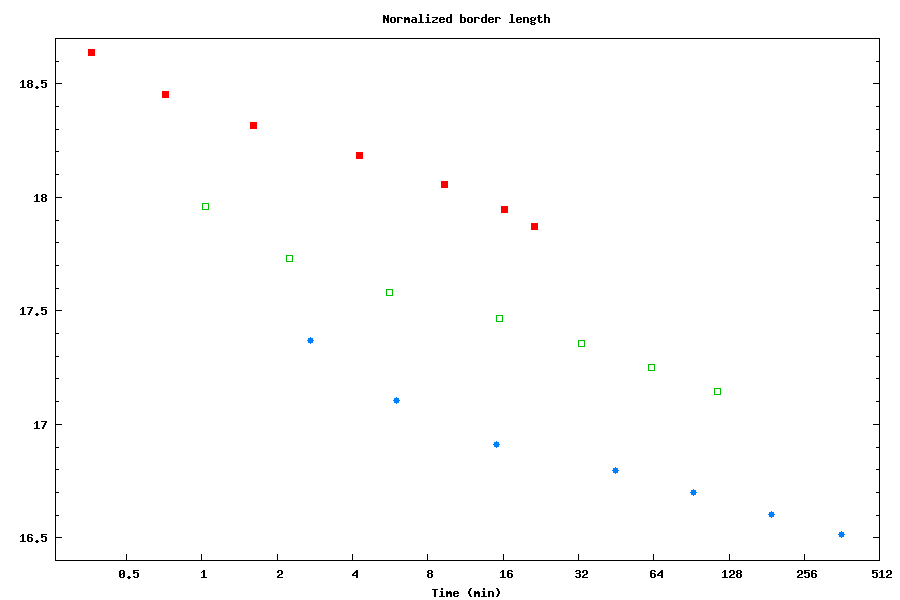
\includegraphics{merge/gplusmasks/bl}
\caption{\label{fig:gplus_blm}%
  Normalized border length per masking step of layouts produced by Greedy with
  $Q=20\,000$ ({\tiny $\times$}) and \Greedyplus\ with $Q=950$
  ({\tiny $\boxdot$}) for a $500\times 500$ chip with border length
  minimization. Both algorithms used $0$-threading and were followed by two
  passes of re-embedding optimization with Sequential.}
\end{figure}

\begin{table}[t!]\centering
\caption{\label{tab:gplus_reptx}
  Normalized border length (NBL) of layouts produced by Row-Epitaxial and
  \Greedyplus\ (both with $0$-threading) on random chips in approximately the
  same amount of time. (total time in minutes including two passes of Sequential
  re-embedding optimization). The relative difference in NBL and time between
  the two approaches is shown in percentage.}
\footnotesize{
\begin{tabular}{crrrlrrrlrr}
\vspace{1pt}
                & \multicolumn{3}{c}{Row-Epitaxial and Sequential} & & \multicolumn{3}{c}{\Greedyplus\ and Sequential} & & \multicolumn{2}{c}{Relative} \\ \cline{2-4} \cline{6-8} \cline{10-11}
\vspace{1pt}
Dim.            & Q       & NBL     &  Time & & Q      & NBL     & Time & & NBL       & Time \\
\hline
$300\times 300$ & 10\,000 & 18.0524 &   4.3 & &    300 & {\bf 17.9807} &  4.2 & & $-0.40\%$ &  $-1.24\%$ \\
                & 20\,000 & 17.9430 &   9.5 & &    700 & {\bf 17.6746} &  9.2 & & $-1.50\%$ &  $-2.85\%$ \\
\hline
$500\times 500$ & 10\,000 & 17.3584 &  16.0 & &    450 & {\bf 17.2216} & 16.0 & & $-0.79\%$ &  $-0.40\%$ \\
                & 20\,000 & 17.2502 &  34.7 & &    950 & {\bf 16.9382} & 30.4 & & $-1.81\%$ & $-12.51\%$ \\
\hline
$800\times 800$ & 10\,000 & 16.7176 &  45.6 & &    500 & {\bf 16.6549} & 41.7 & & $-0.38\%$ &  $-8.51\%$ \\
                & 20\,000 & 16.6012 & 100.1 & & 1\,130 & {\bf 16.3175} & 97.7 & & $-1.71\%$ &  $-2.41\%$ \\
\hline
\end{tabular}}
\end{table}

One advantage of \Greedyplus\ is that, unlike Greedy, it is not influenced by
the initial embeddings of the probes. Figure \ref{fig:gplus_blm} shows the
normalized border length of layouts produced by Greedy and \Greedyplus\ with
border length minimization for a selected $500\times 500$ chip with equivalent
numbers $Q$ of candidates per spot (in accordance with Table
\ref{tab:greedycomp_bl}). Because the probes were initially left-most embedded,
Greedy produced a layout in which the border conflicts are concentrated between
steps 7 and 58; starting on step 59, the normalized border length drops steadily
as the embeddings reach their last productive steps. In contrast, \Greedyplus\
produces a layout with a more uniform distribution of conflicts in the final
synthesis steps. In both cases the first masks have relatively few conflicts as
a result of lexicographically sorting the probes. A representation of selected
masks for the layout produced by \Greedyplus\ is shown in Figure
\ref{fig:gplus-bl_masks}. Layers of masked and unmasked regions in masks
$M_1$ to $M_9$ are similar to the ones shown in Figure
\ref{fig:greedy-bl_masks}, although the masks produced by Greedy are
``noisier''. The normalized border length of these layouts are $17.3182$
(Greedy) and $16.9451$ (\Greedyplus).

\begin{figure}[p]\centering
%%
\begin{picture}(435,567)\footnotesize{
\put( -2,439){\makebox(145,128){
\includegraphics{merge/gplusmasks/mask01}}}
\put(147,439){\makebox(145,128){
\includegraphics{merge/gplusmasks/mask02}}}
\put(292,439){\makebox(145,128){
\includegraphics{merge/gplusmasks/mask03}}}
\put( -2,429){\makebox(145, 10){$M_1$}}
\put(147,429){\makebox(145, 10){$M_2$}}
\put(292,429){\makebox(145, 10){$M_3$}}
\put( -2,296){\makebox(145,128){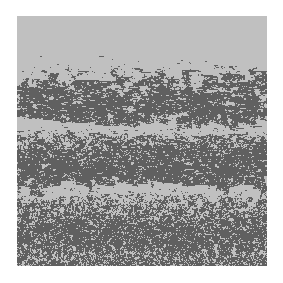
\includegraphics{merge/gplusmasks/mask04}}}
\put(147,296){\makebox(145,128){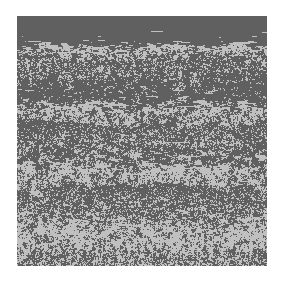
\includegraphics{merge/gplusmasks/mask05}}}
\put(292,296){\makebox(145,128){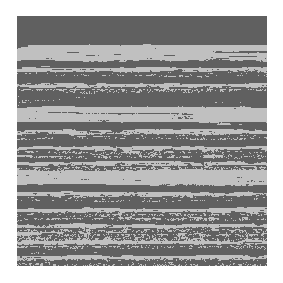
\includegraphics{merge/gplusmasks/mask06}}}
\put( -2,286){\makebox(145, 10){$M_4$}}
\put(147,286){\makebox(145, 10){$M_5$}}
\put(292,286){\makebox(145, 10){$M_6$}}
\put( -2,153){\makebox(145,128){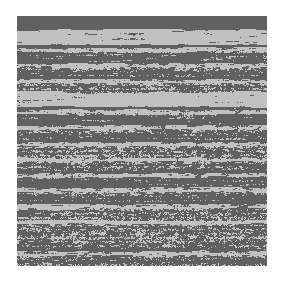
\includegraphics{merge/gplusmasks/mask07}}}
\put(147,153){\makebox(145,128){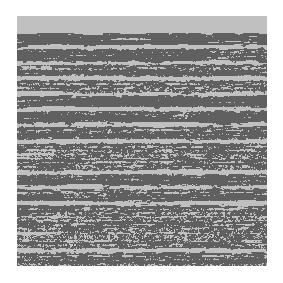
\includegraphics{merge/gplusmasks/mask08}}}
\put(292,153){\makebox(145,128){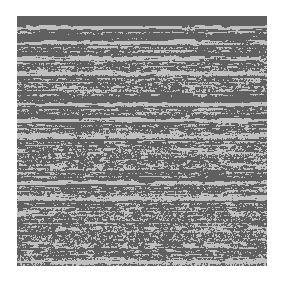
\includegraphics{merge/gplusmasks/mask09}}}
\put( -2,143){\makebox(145, 10){$M_7$}}
\put(147,143){\makebox(145, 10){$M_8$}}
\put(292,143){\makebox(145, 10){$M_9$}}
\put( -2, 10){\makebox(145,128){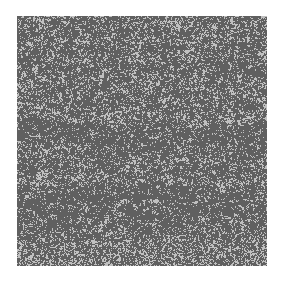
\includegraphics{merge/gplusmasks/mask62}}}
\put(147, 10){\makebox(145,128){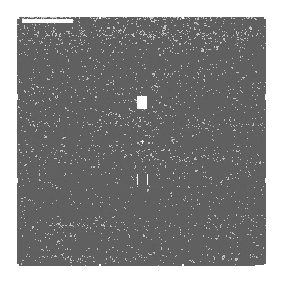
\includegraphics{merge/gplusmasks/mask70}}}
\put(292, 10){\makebox(145,128){
\includegraphics{merge/gplusmasks/mask74}}}
\put( -2,  0){\makebox(145, 10){$M_{62}$}}
\put(147,  0){\makebox(145, 10){$M_{70}$}}
\put(292,  0){\makebox(145, 10){$M_{74}$}}
}\end{picture}
%%
\caption{\label{fig:gplus-bl_masks}%
  Selected masks generated by \Greedyplus\ with border length minimization for a
  $500\times 500$ chip with 25-mer probes embedded in the standard Affymetrix
  deposition sequence. Unmasked (masked) spots are represented by light (dark)
  dots.}
\end{figure}

Finally, we also compare \Greedyplus\ with Row-Epitaxial (Section
\ref{sec:placement_reptx}), which, in terms of border length minimization,
achieves results comparable to Greedy in less time. Table \ref{tab:gplus_reptx}
shows that \Greedyplus\ also outperforms Row-Epitaxial in the same amount of
time (or less). The larger values of $Q$ are used, the greater is the advantage
of \Greedyplus. According to the results of Table \ref{tab:greedyplus_nbl}, the
difference in NBL between \Greedyplus\ and Row-Epitaxial could be even greater
if the former used higher $k$-threading amplitudes.

%%%%%%%%%%%%%%%%%%%%%%%%%%%%%%%%%%%%%%%%%%%%%%%%%%%%%%%%%%%%%%%%%%%%%%%%%%%%%%%%
\section{Summary}
\label{sec:merge_summary}

We have presented a new placement algorithm, called \Greedyplus, that for the
first time places and re-embeds the probes simultaneously. Our results have
shown that \Greedyplus\ outperforms the previously best placement algorithms ---
Row-Epitaxial for border length minimization and Greedy for conflict index
minimization. In terms of CIM, Greedy produces better results when time is
limited but, otherwise, \Greedyplus\ should be the placement algorithm of
choice. In fact, \Greedyplus\ achieves similar results to Greedy by examining
fewer probe candidates per spot and, for this reason, it has the potential for
producing better layouts.

\subsection{Future work}

The fact that \Greedyplus\ does not outperform Greedy so easily in terms of CIM
as it does in terms of BLM could be explained by the fact that probes are sorted
lexicographically, which increases the chances of finding candidates that have
similar prefixes but not good ``matches'' for the middle part of the embeddings.
Greedy has an advantage since it looks at more candidates in the
lexicographically sorted list of probes. One possibility that could improve the
results of \Greedyplus\ is to sort the list of probes with an emphasis on the
middle bases. Although this is technically possible, with our current
implementation of OSPE it would result in an increase in running time because
consecutive candidates would then be unlikely to have a common prefix, requiring
the dynamic programming matrix to be entirely re-computed for each probe
considered. We leave as an open problem the question of finding an ordering of
the probes with an emphasis on the middle bases and an implementation of OSPE in
such a way that consecutive candidates can be examined quickly by skipping the
computation of identical rows of the matrix.
